% !TeX TS-program = xelatex

\documentclass[dvipsnames]{beamer}
\usetheme{metropolis}

\usepackage{multicol}

\usepackage{ragged2e} % who justifies the text
\usepackage{xecolor}
\usepackage{amsmath}
%\usefonttheme[onlymath]{serif} %Change the math font

\usepackage{tabularx}
\usepackage{booktabs}
\usepackage[style=numeric,sorting=ynt]{biblatex}
\addbibresource{references.bib}
\usepackage{xepersian}
\settextfont{Vazir}
\setlatintextfont{Roboto}

%---------------------------------------------------------------------------------
% Seetings to force Beamer works with Xepersian and RTL typesetting
%---------------------------------------------------------------------------------
%\raggedleft

% For right to left lists (itemize and enumerate)
\makeatletter
\newcommand{\RTList}{\raggedleft\rightskip\@totalleftmargin}
\makeatother
% Correct the bullet for RTL texts
\setbeamertemplate{itemize item}{\scriptsize\raise1.25pt%
 \hbox{\donotcoloroutermaths$\blacktriangleleft$}} 

% To force beamer use numbering in captions
\setbeamertemplate{caption}[numbered]{}% Number float-like environments

\setbeamertemplate{footline}[frame number]
\setbeamertemplate{section in toc}[circle]
\setbeamertemplate{blocks}[rounded][shadow=true]
\setbeamercolor{block body}{bg=lightgray}
\setbeamercolor{headline}{bg=orange}
\setbeamersize{text margin left=1cm,text margin right=1cm}

\setbeamertemplate{headline}
{
		\begin{beamercolorbox}{section in head/foot}
				\vspace{2pt}\insertnavigation{\paperwidth}\vspace{2pt}
		\end{beamercolorbox}
}

%---------------------------------------------------------------------------------
% To force beamer use numbering in captions
\setbeamertemplate{caption}[numbered]{}% Number float-like environments

\setbeamertemplate{footline}
{%
	\leavevmode%
	\hbox{%
		\begin{beamercolorbox}[wd=.333333\paperwidth,ht=2.25ex,dp=1ex,center]{author in head/foot}%
			\usebeamerfont{author in head/foot}\insertshortauthor%
		\end{beamercolorbox}%
		\begin{beamercolorbox}[wd=.333333\paperwidth,ht=2.25ex,dp=1ex,center]{title in head/foot}%
			\usebeamerfont{title in head/foot}\insertshorttitle%
		\end{beamercolorbox}%
		\begin{beamercolorbox}[wd=.333333\paperwidth,ht=2.25ex,dp=1ex,right]{date in head/foot}%
			\usebeamerfont{date in head/foot}\insertsection\hspace*{2em}
			\insertframenumber~ از \inserttotalframenumber{} \hspace*{2ex}%
		\end{beamercolorbox}
	}%
}
\setbeamertemplate{section in toc}[circle]
\setbeamertemplate{blocks}[rounded][shadow=true]
\setbeamercolor{block title}{bg=orange}
\setbeamercolor{block body}{bg=lightgray}
\setbeamersize{text margin left=1cm,text margin right=1cm}
\setbeamertemplate{frametitle continuation}{\insertcontinuationcount}

%---------------------------------------------------------------------------------
\title{مجازی‌سازی قطعی کارکردهای شبکه}
\subtitle{}
\author{پرهام الوانی}
\institute{%
		دانشکده مهندسی کامپیوتر\\
		دکتر بهادر بخشی
}
\date{\today}
\titlegraphic{\vspace{4.5cm}\flushleft
\includegraphics[height=50pt]{images/logo}}

\begin{document}

\makeatletter

\setbeamertemplate{title}{%
	\linespread{1.0}%
	\inserttitle%
	\par%
	\vspace*{0.5em}
}
\setbeamertemplate{subtitle}{%
	\insertsubtitle%
	\par%
	\vspace*{0.5em}
}

\AtBeginSection[]
{%
	\begin{frame}{فهرست}
		\tableofcontents[currentsection]
	\end{frame}
	\begin{frame}
		\begin{center}
			\insertsectionnumber. \insertsection%
		\end{center}
		\usebeamertemplate*{title separator}
	\end{frame}
}

\makeatother


\begin{persian}
	%------------------------------------------
	% Title frame (0)
	%------------------------------------------
	{%
		\setbeamertemplate{footline}{}
		\begin{frame}
			\titlepage%
		\end{frame}
	}

	%-------------------------------------------------------------------------------
	\begin{frame}{فهرست}
		\tableofcontents[pausesections]
	\end{frame}

	%-------------------------------------------------------------------------------
	\section{مجازی‌سازی کارکردهای شبکه}

	%-------------------------------------------------------------------------------
	\begin{frame}{شبکه‌های سنتی}
		\begin{itemize}\RTList{}
			\justifying
			\item
						یک سرویس شبکه به صورت تعدادی
						\textcolor{Orange}{کارکرد مشخص}
						که ترافیک با
						\textcolor{Orange}{ترتیب مشخصی}
						از آن ها عبور می‌کند، تعریف می‌شود.
			\item
						کارکردهای شبکه به صورت سخت‌افزار و نرم‌افزار اختصاصی تهیه شده
						از سازندگان مختلف استفاده می‌شوند.
			\item
						کارکردها باید در \textcolor{LimeGreen}{مکان} مناسب در شبکه قرار گیرند و ترافیک به سمت
						آن‌ها \textcolor{LimeGreen}{هدایت} شود.
		\end{itemize}
	\end{frame}

	%-------------------------------------------------------------------------------
	\begin{frame}{شبکه های سنتی}
		\begin{itemize}\RTList{}
			\justifying
			\item
						افزایش نیازمندی به سرویس‌های
						\textcolor{Orange}{متنوع}
						با
						\textcolor{LimeGreen}{عمرکوتاه}
						و
						\textcolor{Cyan}{نرخ بالای ترافیک}
						\begin{itemize}\RTList{}
							\item خریداری، انبارداری و استقرار سخت‌افزارهای اختصاصی
							\item افزایش هزینه‌های خرید، آموزش و انبارداری
							\item کاهش فضای فیزیکی
							\item سربار آموزش کارکنان
							\item محدودیت نوآوری در سخت‌افزار و سرویس
						\end{itemize}
		\end{itemize}
		\begin{block}{}
			\centering
			\lr{Network Functions Virtualization}\\
			مجازی‌سازی کارکردهای شبکه
		\end{block}
	\end{frame}

	%-------------------------------------------------------------------------------
	\begin{frame}{شبکه های سنتی}
		\begin{itemize}\RTList{}
			\justifying
			\item ترافیک کاربر باید از تعدادی کارکرد شبکه به ترتیب معینی عبور کند.
			\item کارکردها به صورت سخت‌افزاری به یکدیگر متصل هستند و ترافیک با استفاده از جداول مسیریابی به سمت آن‌ها هدایت می‌شود.
			\item نیاز به تغییر همبندی سریع و یا مکان کارکردها برای سرویس‌دهی بهتر
						\begin{itemize}\RTList{}
							\item استقرار و تغییر ترتیب کارکردها دشوار است
							\item امکان رخدادن خطاهای متعدد
						\end{itemize}
		\end{itemize}
		\begin{block}{}
			\centering
			\lr{Service Function Chaining}\\
			زنجیره‌سازی کارکرد سرویس
		\end{block}
	\end{frame}

	%-------------------------------------------------------------------------------
	\begin{frame}{راهکار \lr{NFV}}
		\begin{itemize}\RTList{}
			\justifying
			\item مجازی‌سازی کارکردهای شبکه
						\begin{itemize}\RTList{}
							\item اواخر سال ۲۰۱۲، \lr{ETSI NFV ISG} توسط هفت اپراتور جهانی شبکه تأسیس شد.
							\item اکنون بیش از 250 سازمان با آن همکاری می‌کنند.
							\item اجرای کارکردها بر روی سرورهای استاندارد با توان بالا به وسیله مجازی‌سازی کارکردها
										\begin{itemize}\RTList{}
											\item کاهش نیاز به تجهیزات سخت‌افزاری خاص منظوره
											\item اشتراک گذاری منابع بین کارکرد‌ها
											\item کاهش هزینه‌های تجهیزات و مصرف انرژی از طریق تجمیع کارکردها
										\end{itemize}
						\end{itemize}
		\end{itemize}
	\end{frame}

	%-------------------------------------------------------------------------------
	\begin{frame}{راهکار \lr{NFV}}
		\begin{itemize}\RTList{}
			\justifying
			\item زنجیره‌سازی کارکرد سرویس
						\begin{itemize}\RTList{}
							\item امکان تعریف زنجیره کارکردها به صورت پویا و بدون تغییر در زیرساخت فیزیکی
							\item قابل اجرا بر بستر \textcolor{LimeGreen}{شبکه‌های سنتی} یا \textcolor{Orange}{نرم‌افزار بنیان}
							\item \lr{RFC 7665}
						\end{itemize}
		\end{itemize}
	\end{frame}

	%-------------------------------------------------------------------------------
	\begin{frame}{راهکار \lr{NFV}}
		\begin{itemize}\RTList{}
			\justifying
			\item زنجیره‌های مرتب تمام
			\item زنجیره‌های مرتب جزئی
		\end{itemize}
		\begin{center}\begin{figure}
				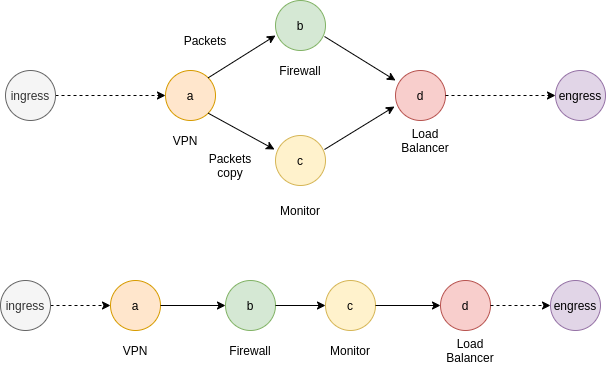
\includegraphics[scale=0.3]{images/partially-totally-sfc.png}
				\caption{زنجیره‌های مرتب جزئی و کامل}
				\vspace*{-1cm}
		\end{figure}\end{center}
		\begin{latin}
		\noindent\rule{1cm}{0.4pt}\\
		\tiny\fullcite{Yang2021}
		\end{latin}
	\end{frame}

	%-------------------------------------------------------------------------------
	\begin{frame}{راهکار \lr{NFV}}
		\begin{center}\begin{figure}
				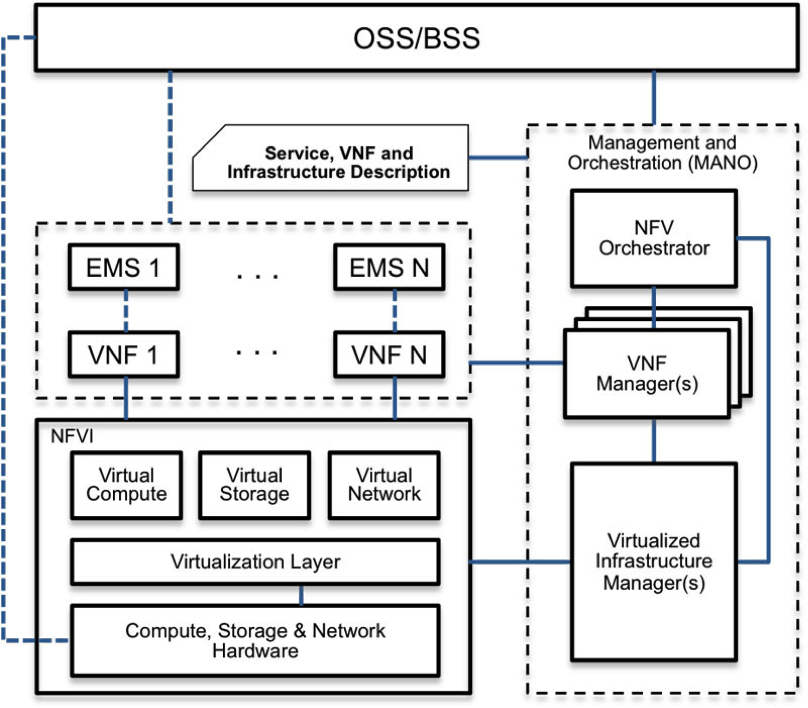
\includegraphics[scale=0.5]{images/nfv-arch.png}
				\caption{معماری سطح بالای مجازی‌سازی کارکردهای شبکه}
			\end{figure}\end{center}
	\end{frame}

	%-------------------------------------------------------------------------------
	\begin{frame}{راهکار \lr{NFV}}
		\begin{itemize}\RTList{}
			\justifying
			\item \lr{NFVO} وظیفه‌ی استقرار زنجیره‌های کارکرد سرویس را برعهده دارد.
			\item \lr{VNFM} مسئول چرخه‌ی زندگی کارکردهای مجازی شبکه می‌باشد.
		\end{itemize}
	\end{frame}

	%-------------------------------------------------------------------------------
	\begin{frame}{تخصیص منابع}
		\begin{itemize}\RTList{}
			\justifying
			\item
						جایگذاری کارکردهای مجازی شبکه به همراه مسیریابی ترافیک\\
						\begin{center}\footnotesize\lr{VPTR: VNF Placement and Traffic Routing}\end{center}
			\item
						جایگذاری کارکردهای مجازی شبکه\\
						\begin{center}\footnotesize\lr{VNFP: VNF Placement}\end{center}
			\item
						مسیریابی ترافیک\\
						\begin{center}\footnotesize\lr{TRR: Traffic Routing}\end{center}
			\item
						بازاستقرار و تثبیت کارکردهای مجازی شبکه\\
						\begin{center}\footnotesize\lr{VRC: VNF Redeployment and Consolidation}\end{center}
		\end{itemize}
	\end{frame}

	%-------------------------------------------------------------------------------
	\begin{frame}{اهداف}
		\begin{itemize}\RTList{}
			\justifying%
			\item هزینه
						\begin{itemize}\RTList{}
							\item مساله‌ی پایه‌ای در بحث تخصیص منابع
							\item وجود جواب با برآورده شدن محدودیت‌های نودها و لینک‌ها
							\item \lr{NP-Hard}
						\end{itemize}
			\item \textcolor{LimeGreen}{کیفیت سرویس}
						\begin{itemize}\RTList{}
							\item \textcolor{Orange}{تاخیر}
						\begin{itemize}\RTList{}
							\item انتشار
							\item انتقال
							\item صف
							\item پردازش
						\end{itemize}
							\item دسترسی پذیری
						\end{itemize}
		\end{itemize}
	\end{frame}

	%-------------------------------------------------------------------------------
	\begin{frame}{اهمیت تاخیر}
		\begin{itemize}\RTList{}
			\justifying%
			\item کیفیت سرویس انتها به انتها یک زنجیره در واقع معیار کارآیی است که توسط کاربران احساس می‌شود.
			\item ظهور اینترنت اشیا و شبکه‌های نسل پنجم
			\begin{itemize}\RTList{}
				\item \lr{Tactile Internet}
				\item شبکه‌های باتاخیر بسیار کم
			\end{itemize}
		\end{itemize}
	\end{frame}

	%-------------------------------------------------------------------------------
	\begin{frame}{مدل‌سازی تاخیر}
		\begin{itemize}\RTList{}
			\justifying%
			\item برای محاسبه تاخیر نیاز به مدل‌سازی می‌باشد.
			\item می‌توان تاخیر را ثابت فرض کرده یا آن را به صورت معین در نظر گرفت.
			\item تاخیر \textcolor{LimeGreen}{تصادفی}
			\begin{itemize}\RTList{}
				\item تئوری صف: حالت میانه را پیدا می‌کند.
				\item \textcolor{Orange}{\lr{Network Calculus}}: بدترین حالت را پیدا می‌کند و می‌بایست مدل مناسب با کمترین فاصله را بدست آورد.
			\end{itemize}
		\end{itemize}
	\end{frame}


	%-------------------------------------------------------------------------------
	\section{شبکه‌های قطعی}

	%-------------------------------------------------------------------------------
	\begin{frame}{مقدمه}
		\begin{itemize}\RTList{}
			\justifying%
			\item حضور کاربردهای بلادرنگ بسیار حساس به تاخیر و خرابی
			\begin{itemize}\RTList{}
			  	\item مهاجرت از شبکه‌های خاص‌منظوره به شبکه‌های \lr{IP}
				\item تاخیر قطعی در مقابل تاخیر احتمالی
			\end{itemize}
			\item عدم قطعیت ذاتی شبکه‌های فعلی
			\begin{itemize}\RTList{}
				\item الگوریتم‌های زمان‌بندی
				\item ازدحام
				\item خرابی
				\item ...
			\end{itemize}
			\item نیاز به ایجاد قطعیت در معماری شبکه
		\end{itemize}
	\end{frame}

	%-------------------------------------------------------------------------------
	\begin{frame}{شبکه‌‌سازی حساس به زمان \lr{(Time Sensitive Networking)}}
		\begin{itemize}\RTList{}
			\justifying%
			\item کارگروه \lr{IEEE 802.1 TSN}
			\item تمرکز بر لایه پیوند داده
			\item جریان \lr{TSN}: یک ارتباط شبکه‌ای تک‌پخشی یا چند‌پخشی از یک ایستگاه انتهایی به یک ایستگاه انتهایی دیگر
			\begin{itemize}\begin{latinitems}
				\item Flow Concept
				\item Flow Synchronization
				\item Flow Management
				\item Flow Control
				\item Flow Integrity
			\end{latinitems}\end{itemize}
		\end{itemize}
	\end{frame}

	%-------------------------------------------------------------------------------
	\begin{frame}{شبکه‌سازی قطعی (\lr{Deterministic Networking})}
		\begin{itemize}\RTList{}
			\justifying%
			\item کارگروه \lr{IETF DetNet}
			\item تمرکز بر لایه شبکه
			\item جریان‌های \lr{DetNet} بر اساس کلاس‌های کیفیت سرویس مشخص می‌شوند.
			\item اهداف
			\begin{itemize}\RTList{}
				\item کران معین برای تاخیر
				\item کران معین تغییرات تاخیر
				\item کمترین میزان از دست رفتن بسته
			\end{itemize}
		\end{itemize}
	\end{frame}

	%-------------------------------------------------------------------------------
	\begin{frame}{معماری شبکه‌سازی قطعی}
		\begin{itemize}\RTList{}
			\justifying%
			\item کیفیت سرویس در شبکه‌های قطعی:
			\begin{itemize}\RTList{}
			  \item کران بالا و پایین برای تاخیر انتها به انتها از مبدا به مقصد، تغییرات تاخیر کران‌دار، ارسال زمان‌دار
			  \item نسبت از دست رفتن بسته‌ها تحت فرض‌های مختلف
			  \item کران بالا برای بسته‌های خارج از ترتیب
			\end{itemize}
		  \item تنها دغدغه در شبکه‌سازی قطعی بدترین حالت‌ها می‌باشند.
		  \item اینجا حالت‌های میانگین و ... از اهمیت کمی برخوردار هستند.
		  \item تکنیک‌های برآورده ساختن نیازمندی‌های کیفیت سرویس
		  \begin{itemize}\RTList{}
			\item تخصیص منابع
			\item حفاظت از سرویس
			\item مسیرهای صریح
		  \end{itemize}
		\end{itemize}
	\end{frame}

	%-------------------------------------------------------------------------------
	\begin{frame}{معماری شبکه‌سازی قطعی}
		\begin{itemize}\RTList{}
			\justifying%
			\item تخصیص منابع
			\begin{itemize}\RTList{}
			  \item بدست آوردن کیفیت سرویس با از بین بردن یا کاهش اثر از دست رفتن بسته‌ها در اثر ازدحام
			  \item کاهش تغییرات تاخیر
			\end{itemize}
		  \item حافظت از سرویس با تحمل یا از بین بردن از دست رفتن بسته‌ها در اثر خرابی تجهیزات
		  \begin{itemize}\RTList{}
			\item ارسال به ترتیب بسته‌ها
			\item تکرار بسته‌ها
			\item کد کردن بسته‌ها
		  \end{itemize}
		  \item مسیرهای صریح در اثر تغییرات بلافلاصه تغییر نمی‌کند و تلاش می‌کند تا حد امکان تغییر نکند.
		\end{itemize}
	\end{frame}

	%-------------------------------------------------------------------------------
	\begin{frame}{معماری شبکه‌سازی قطعی}
		\begin{center}\begin{figure}
			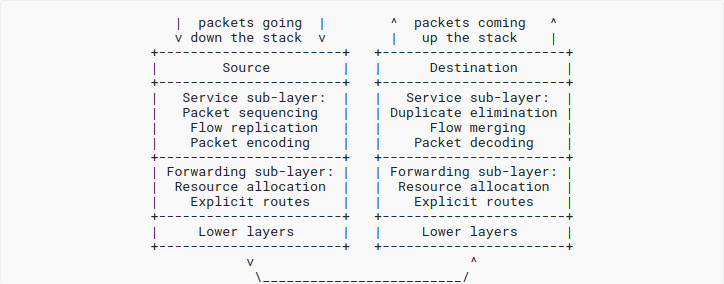
\includegraphics[scale=0.4]{images/detnet-stack.png}
			\caption{معماری پشته شبکه‌های قطعی}
		\end{figure}\end{center}
	\end{frame}

	%-------------------------------------------------------------------------------
	\begin{frame}{آشنایی با \lr{Network Calculus}}
		\begin{itemize}\RTList{}
			\justifying%
			\item دیود \((R \cup +\infty, \wedge, +)\)
			\item جمع تبدیل به محاسبه‌ی \lr{infimum} می‌شود.
			\item ضرب به جمع تبدیل می‌شود.
			\[ (3\wedge4) + 5 = (3 + 5) \wedge (4 + 5) = 8 \wedge 9 = 8 \]
			\item پیچیش کمینه - جمع
			\[ (f \otimes g)(t) = \int_{0}^{t} f(t-s)g(s)ds \]
		\end{itemize}
	\end{frame}

	%-------------------------------------------------------------------------------
	\begin{frame}{آشنایی با \lr{Network Calculus}}
		\begin{itemize}\RTList{}
			\justifying%
		  \item \textcolor{LimeGreen}{منحنی ورودی،}
				جریان \(R\) با \( \alpha(.) \) محدود شده است.
			\[ R(t) - R(s) \le \alpha(t - s) \]
		  \item \textcolor{Orange}{منحنی سرویس}
				برای جریان وروردی \(R\) و جریان خروجی \(R^{*}\) برابر با \(b\):
			\[ R^{*} \ge R \otimes b \]
		\end{itemize}
	\end{frame}

	%-------------------------------------------------------------------------------
	\section{مرور ادبیات}

	%-------------------------------------------------------------------------------
	\begin{frame}{مرجع~\cite{Qu2016}}
		\begin{itemize}\RTList{}
			\justifying%
			\item مساله‌ی زمان‌بندی سرویس‌های شبکه
			\item سرویس‌های شبکه در قالب تعداد کارکرد مجازی با عمرمحدود
			\item کارکردهای مجازی شبکه به صورت \lr{store-and-foward} عمل می‌کنند.
			\item تاخیر انتقال و تاخیر پردازش
			\item این مقاله محدودیت پردازش برای نودها و ظرفیت برای لینک‌ها را در نظر گرفته است.
			\item کارکردها می‌توانند میزان جریان عبوری را تغییر دهند. مثلا دیوار آتش می‌تواند بسته‌ها را عبور ندهد.
		\end{itemize}
		\begin{latin}
		\noindent\rule{1cm}{0.4pt}\\
		\scriptsize\fullcite{Qu2016}
		\end{latin}
	\end{frame}

	%-------------------------------------------------------------------------------
	\begin{frame}{مرجع~\cite{Li2017}}
		\begin{itemize}\RTList{}
				\justifying%
				\item ارائه‌ی یک چهارچوب مدیریتی براساس مدل تاخیر ارائه شده
				\item تاخیر پردازش برای تعداد مشخصی نمونه از کارکرد
				\item دسته‌بندی کارکردها
				\begin{itemize}\RTList{}
						\item وابسته به اندازه بسته (\lr{exponential})
						\item مستقل از اندازه بسته (\lr{deterministic})
				\end{itemize}
		\end{itemize}
		\begin{latin}
		\noindent\rule{1cm}{0.4pt}\\
		\scriptsize\fullcite{Li2017}
		\end{latin}
	\end{frame}

	%-------------------------------------------------------------------------------
	\begin{frame}{مرجع~\cite{Yang2019}}
		\begin{itemize}\RTList{}
				\justifying%
				\item تاخیر انتقال و تاخیر پردازش
				\item در نظر گرفتن زنجیره‌های مرتب جزئی و تاثیر آن‌ها بر تاخیر
				\item قطعه قطعه کردن زنجیره‌های مرتب جزئی برای تبدیل آن‌ها به تعدادی زنجیره مرتب کامل
		\end{itemize}
		\begin{latin}
		\noindent\rule{1cm}{0.4pt}\\
		\scriptsize\fullcite{Yang2019}
		\end{latin}
	\end{frame}

	%-------------------------------------------------------------------------------
	\begin{frame}{مرجع~\cite{Huang2019}}
		\begin{itemize}\RTList{}
				\justifying%
				\item تاخیر انتقال ثابت در نظر گرفته شده است.
				\item زنجیره‌ها نیازمندی تاخیر انتها به انتها دارند.
		  		\item مساله‌ی بهینه‌سازی چند دوره‌ای
				\item به اشتراک گذاری نمونه‌ها
				\item گسترش عرضی و طولی
				\item عدم توانایی در نظر گرفتن همه این شرایط در مساله‌ی بهینه‌سازی
		\end{itemize}
		\begin{latin}
		\noindent\rule{1cm}{0.4pt}\\
		\scriptsize\fullcite{Huang2019}
		\end{latin}
	\end{frame}

	%-------------------------------------------------------------------------------
	\begin{frame}{مرجع~\cite{Duan2018}}
		\begin{itemize}\RTList{}
				\justifying%
				\item یافتن کران پایین سرویس‌دهی و استفاده از \lr{Network Calculus} برای زنجیره‌سازی آن‌ها
				\item در نظر گرفتن نمایه \lr{Latency Rate (LR)} برای سرویس‌ها
				\[ P[r, \theta](t) = \max\{0, r(t - \theta)\} \]
				\[ \theta: latency \]
				\[ r: rate \]
		\end{itemize}
		\begin{latin}
		\noindent\rule{1cm}{0.4pt}\\
		\scriptsize\fullcite{Duan2018}
		\end{latin}
	\end{frame}

	%-------------------------------------------------------------------------------
	\section{مساله‌ی پیشنهادی}

	%-------------------------------------------------------------------------------
	\begin{frame}{مساله‌ی پیشنهادی}
		\begin{itemize}\RTList{}
				\justifying%
				\item نیازمندی‌های شبکه‌های قطعی
				\item کران بالای پارامترهای غیرقطعی
				\item مجازی‌سازی کارکردهای شبکه
		\end{itemize}
	\end{frame}

	%-------------------------------------------------------------------------------
	\begin{frame}{مساله‌ی پیشنهادی}
		\begin{block}{}
			\centering
			جایگذاری زنجیره‌هایی با کارکردهای قطعی در زیرساخت مجازی‌سازی شبکه
		\end{block}
	\end{frame}

	%-------------------------------------------------------------------------------
	\begin{frame}{روش‌ پیشنهادی}
		\begin{enumerate}\RTList{}
				\justifying%
				\item مدل‌سازی تاخیر با استفاده از \lr{Network Calculus} برای محاسبه کران‌های بالا
				\item مدل‌سازی مساله‌ی بهینه‌سازی
				\item تخمین مساله‌ی بهینه‌سازی با یادگیری تقویتی و ...
		\end{enumerate}
	\end{frame}

	%-------------------------------------------------------------------------------
	\begin{frame}[allowframebreaks]{مراجع}
		\begin{latin}
		\printbibliography[title=مراجع]
		\end{latin}
	\end{frame}

\end{persian}
\end{document}
